\documentclass[aps,twocolumn,floats,nofootinbib,prl]{revtex4}
\usepackage{graphics,graphicx,epsfig}
\usepackage{amssymb,color}
\usepackage{epsf,epstopdf,wrapfig}
\usepackage {amsmath}
%\usepackage{axodraw}

\newcommand{\abs}[1]{|#1|}
\newcommand{\av}[1]{\langle{#1}\rangle{}}
\newcommand{\beq}{\begin{equation}}
\newcommand{\eeq}{\end{equation}}
\newcommand{\beqn}{\begin{eqnarray}}
\newcommand{\eeqn}{\end{eqnarray}}
\newcommand {\e}[1]{\mathrm{~#1}}    
\newcommand {\E}[1]{\cdot 10^{#1}}		
\begin{document}

\title{PCA meets RG}

\author{Serena Bradde$^a$ and William Bialek$^{a,b}$}

\affiliation{$^a$Initiative for the Theoretical Sciences, The Graduate Center, City University of New York, 365 Fifth Ave., New York, New York 10016\\
$^b$Joseph Henry Laboratories of Physics, and Lewis--Sigler Institute for Integrative Genomics, Princeton University, Princeton NJ 08544}

\date{\today}

\begin{abstract}
\textcolor{red}{Come back and write an abstract at the end.}
\end{abstract}

\maketitle

Many of the most interesting phenomena in the world around us emerge from interactions among many degrees of freedom.  In the era of ``big data,'' we are encouraged to think about these systems more explicitly, describing the state of the system as a point in a space with many dimensions:  the state of a cell is defined by the expression level of many genes, the state of a financial market is defined by the prices of many stocks, and so on.  One standard approach to the analysis of these high dimensional data is to look for a linear projection onto a lower dimensional space that captures most of the (interesting) variations.  Quantitatively, the best projection is found by diagonalizing the covariance matrix, which decomposes the variations into modes that are independent at second order; these are the principal components (PCs), and the method is called principal components analysis (PCA).  In favorable cases, very few modes will capture most of the variance, but it is much more common to find that the eigenvalues of the covariance matrix form a more continuous spectrum, so that any sharp  division between important and unimportant dimensions would be arbitrary. 

%\textcolor{red}{[No attempts yet at references, which will be crucial.   It would be great to have a schematic figure---maybe a covariance matrix and its spectrum, contrast gapped and continuous cases, show a cutoff, compare with a physics example and momentum cutoff ... .]}

For physical systems in thermal equilibrium, it again is the case that the most interesting phenomena emerge from interactions among many degrees of freedom.  But here we have a quantitative language for describing this emergence.  In the classical view, we make precise models of the interactions on a microscopic scale, and then statistical mechanics is about calculating the implications of these interactions for the macroscopic behavior of matter.   In the modern view, we admit that our microscopic description itself is approximate, incorporating ``effective interactions'' mediated by degrees of freedom that we might not want to describe explicitly, and that the distance scale at which we draw the boundary between explicit and implicit description also is arbitrary.  Attention shifts from the precise form of our model to the way in which this model evolves as we move the boundary between degrees of freedom that we describe and those that we ignore; the evolution through the space of possible models is described by the renormalization group (RG).  A central result of the RG is that many detailed features of models on a microscopic scale disappear as we coarse--grain our description out to the macroscopic scale, and that in many cases we are left with only a few terms in our models, the ``relevant operators.''  Thus, some of the success of simple models in describing the world comes not from an inherent simplicity, but rather from the fact that many macroscopic behaviors are insensitive to microscopic details (irrelevant operators).  

The RG approach to statistical physics suggests that systems in which PCA fails to yield a clean separation between high variance and low variance modes may nonetheless be simplified.  Indeed, in a system where the many degrees of freedom live on a lattice, with translation invariant interactions, the eigenmodes of the covariance matrix (principal components) are Fourier modes, and typically we find that the variance of each mode decreases monotonically but smoothly with the wavelength of these modes.  In the momentum space implementation of RG, we put a cutoff on the wavelength, and ask what happens to the joint distribution of the remaining variables as we move this cutoff to progressively longer wavelengths, averaging over the low variance modes.  In this language, the RG is about what happens as we vary the arbitrary distinction between high variance PCs that we keep, and low variance PCs that we ignore.    The goal of this paper is to make this connection between PCA and RG more clear, and more general, so that we can construct RG approaches to the analysis of more complex high dimensional systems.

Familiar formulations of the RG make very explicit use of translation invariance (in the momentum space version) or the locality of interactions (in the real space version), but in more complex systems we cannot lean on these  simplifications.  We argue that the notion of relevant and irrelevant operators can be recast, at least perturbatively, in terms of the eigenvalue spectrum of a matrix that becomes the covariance matrix in the limit of nearly Gaussian distributions.  This argument suggests conditions under which we can simplify our description of complex, high dimensional systems, well beyond the class of problems described by equilibrium statistical physics.

Let us imagine that the system we are studying is described by a set of variables $\phi_1, \, \phi_2, \, \cdots ,\, \phi_N \equiv \{\phi_{\rm i}\}$, where the dimensionality $N$ is large.  For the purposes of this discussion, ``describing the system'' means  writing down the joint probability of all $N$ variables, $P(\{\phi_{\rm i}\})$.  For simplicity we define these variables so that they have zero mean, and we'll assume that positive and negative fluctuations are equally likely (though this is not essential).    We start with the guess that the fluctuations are nearly Gaussian, so we can write
\begin{equation}
P(\{\phi_{\rm i}\}) = \frac{1}{Z}\exp\left[ - \frac{1}{2}\sum_{{\rm i},{\rm j}} \phi_{\rm i} K_{\rm ij} \phi_{\rm j} - \frac{1}{4!}\sum_{\rm i} g_{\rm i} \phi_{\rm i}^4 + \cdots \right] ,
\label{P1}
\end{equation}
where the coefficients $g_{\rm i}$ allow us to describe weak kurtosis of each individual variable, and in the limit $g_{\rm i} = 0$ the matrix $K_{\rm ij}$ is the inverse of the covariance matrix
\begin{equation}
C_{\rm ij} = \langle \phi_{\rm i}\phi_{\rm j}\rangle .
\end{equation}
It may be useful to note that the probability distribution in Eq (\ref{P1}) is the maximum entropy, and hence least structured,  model consistent with the full covariance matrix and the kurtosis  of each individual variable; in this sense it is a minimal model. We start  in the Gaussian approximation and explore perturbations around this case.  

It is useful to write the eigenvalues $\lambda_\mu$ and eigenvectors $\{u_{\rm i}(\mu )\}$ of the symmetric matrix $K$,
\begin{equation}
\sum_{\rm j} K_{\rm ij} u_{\rm j}(\mu )  = \lambda_\mu u_{\rm i}(\mu ),
\end{equation}
with the usual normalization and orthogonality conditions when all the eigenvalues are distinct,
\begin{eqnarray}
\sum_{\rm i} u_{\rm i}(\mu ) u_{\rm i}(\mu' ) &=&\delta_{\mu\mu'}
\label{normA}\\
\sum_\mu u_{\rm i}(\mu )u_{\rm j}(\mu ) &=& \delta_{\rm ij} .
\end{eqnarray}
The eigenvectors for $\lambda\neq0$, on the other hand, satisfy
\begin{equation}\label{eqn:eigvect}
\sum_{\rm i} u_{\rm i}(\mu ) =0\,.
\end{equation}
So that the variations in $\{\phi_{\rm i}\}$ can be decomposed into modes $\{\tilde\phi_\mu\}$,
\begin{equation}
\phi_{\rm i} = \sum_\mu u_{\rm i} (\mu )\tilde\phi_\mu \,.
\end{equation}
In the regime of zero kurtosis $g_{\rm i} = 0$, then these modes are exactly the principal components.
The Gaussian term in the probability distribution becomes
\begin{equation}
  \frac{1}{2}\sum_{{\rm i},{\rm j}} \phi_{\rm i} K_{\rm ij} \phi_{\rm j}  =   \frac{1}{2}\sum_\mu \lambda_\mu \tilde\phi_\mu^2 ,
  \end{equation}
and hence the variance of each mode is given by $\langle \tilde\phi_\mu^2\rangle = 1/\lambda_\mu$.  Importantly this means that the average variance of the individual variables is in this regime
\begin{equation}
\frac{1}{N}\sum_{\rm i}\langle \phi_{\rm i}^2\rangle = \frac{1}{N}\sum_\mu \frac{1}{\lambda_\mu} \rightarrow \int_0^\Lambda d\lambda\, \rho(\lambda ) \frac{1}{\lambda},
\label{meanvar1}
\end{equation}
where in the last step we define the probability distribution of eigenvalues as
\begin{equation}
\rho (\lambda ) = \frac{1}{N}\sum_\mu \delta (\lambda - \lambda_\mu ).
\end{equation}
The density of eigenvalues becomes smooth in the limit of infinite dimensionality, and we emphasize explicitly that the integral is done up to the largest eigenvalue $\Lambda=\max_\mu \{\lambda_\mu\}$.

The essential idea of our approach is to integrate over the modes that have small variance.  This is the standard PCA approach when there is a clear cutoff in the density of eigenvalues between relevant and irrelevant modes. However, in the opposite scenario when the density of eigenvalues decays continuously, this corresponds to restricting our attention only to modes with $\lambda$ {\em less} than some cutoff and observe what happens when the cutoff is varied.  More explicitly, this corresponds to decreasing the limit $\Lambda$ on the integral over eigenvalues, e.g. in Eq (\ref{meanvar1}).  The effect of this renormalization is to reduces the total variance, 
%which sets the scale of variations, and this in turn is related to the units that we use in measuring $\{\phi_{\rm i}\}$.  It 
but it is natural to choose units in which the variance is fixed, and  this implies that as we change the cutoff $\Lambda$ we have to rescale the values of $\phi_{\rm i}$.  So we  replace $\phi_{\rm i} \rightarrow z_\Lambda \phi_{\rm i}$, and we can determine this scale factor by insisting that the mean variance stay fixed:
\begin{eqnarray}
0 &=& \frac{d}{d\Lambda} \left[ \frac{1}{N}\sum_{\rm i}\langle (z_\Lambda\phi_{\rm i})^2\rangle\right]\\
&=& \frac{d}{d\Lambda} \left[\int_0^\Lambda d\lambda\, \rho(\lambda ) \frac{(z_\Lambda)^2}{\lambda}\right]\\
\Rightarrow \frac{d\ln z_\Lambda}{d\ln \Lambda} &=& - \frac{1}{2} \rho(\Lambda ) \left[ \int_0^\Lambda d\lambda\, \rho(\lambda ) \frac{1}{\lambda}\right]^{-1} \label{eqn:zlambda}.
\end{eqnarray}
Thus, as we change the scale of the smallest variance mode that we include in our analysis, we also have to change the scale of the variables $\{\phi_{\rm i}\}$ themselves, and this scaling is determined by the probability distribution of eigenvalues of the (inverse) covariance matrix.

The rescaling of variables determines whether terms such as the quartic $\sim g_{\rm i}$ in Eq (\ref{P1}) will become more or less important as we move the cutoff $\Lambda$.  To begin with, we want to write everything in terms of the rescaled variables.  But, in addition,
%so that 
%\begin{equation}
%\sum_{\rm i} g_{\rm i} \phi_{\rm i}^4 \rightarrow  \sum_{\rm i} z_{\Lambda}^{-4} g_{\rm i} (z_\Lambda \phi_{\rm i})^4 .
%\end{equation}
%Further, 
when we reduce the cutoff, we reduce the number of degrees of freedom in the system.  The average of the quadratic term in the (log) probability distribution is automatically proportional to this effective number of degrees of freedom, \begin{equation}
N_{\rm eff} = N\int_0^\Lambda d\lambda \,\rho(\lambda ),
\end{equation}
and this insures, for example, that the entropy of the probability distribution will be proportional to $N_{\rm eff}$. 
To be sure that this works also for the quartic terms, we write
%, and we always want the log of probability to be proportional to the number of degrees of freedom \textcolor{red}{[maybe this needs explanation! note that it happens automatically for the quadratic term]}.  Thus we write
\begin{eqnarray}
N \sum_{\rm i} g_{\rm i} \phi_{\rm i}^4  = N_{\rm eff} \sum_{\rm i} \tilde g_{\rm i}(z_\Lambda \phi_{\rm i})^4 \Rightarrow
 \tilde g_{\rm i} = z_{\Lambda}^{-4} g_{\rm i} \frac{N}{N_{\rm eff}} .
\end{eqnarray}
Now we can define the scaling dimension of the coefficient $\tilde g_{\rm i}$ given by
\begin{equation}
\frac{d\ln \tilde g_{\rm i} }{d\ln\Lambda} = \rho(\Lambda) \left[  2 \frac{1}{\int_0^\Lambda d\lambda\, \rho(\lambda ) \frac{1}{\lambda}} - \frac{\Lambda}{\int_0^\Lambda d\lambda \,\rho(\lambda )} \right] ,
\label{dG4}
\end{equation}
where we use the equation (\ref{eqn:zlambda}) for the log derivative of the scale factor. Notice that the two terms in equation (\ref{dG4}) are both positive, this means that we can find either sign for the result.  

If the scaling function ${d\ln \tilde g_{\rm i} }/{d\ln\Lambda}$ is positive, then as we decrease the cutoff $\Lambda$  and thus average over more and more of the low variance modes, any small quartic term $\tilde g_{\rm i}$ will become still smaller, and hence the distribution approaches a Gaussian.  This seems to make sense, since when we project onto a (much) lower dimensional space, each of the variables that remains is a weighted sum of many variables, and we might expect the central limit theorem to enforce approximate Gaussianity of the resulting distribution.  

But if the scaling function ${d\ln \tilde g_{\rm i} }/{d\ln\Lambda} < 0$, then as we average over more and more of the lower variance modes, the quartic term becomes more and more important to the structure of the distribution.    To use the language of the RG, under these conditions the quartic term is a relevant operator.  

To see that  our results for the scaling function and the definition of a relevant operator match that in the conventional RG analysis, let's think about a system in which the variables $\phi$ live at positions $\mathbf x$ in a $D$ dimensional Euclidean space.  Then the correlations come from a  ``kinetic energy'' term that enforces similarity among neighbors, 
\begin{equation}
 \frac{1}{2}\sum_{{\rm i},{\rm j}} \phi_{\rm i} K_{\rm ij} \phi_{\rm j}  \rightarrow \frac{1}{2}\int d^D x \left[ {\mathbf\nabla} \phi({\mathbf x}) \right]^2 .
\end{equation}
The eigenvectors of $K$ are then Fourier modes, as noted above, indexed by a wave vector $\mathbf k$, and the associated eigenvalue is $\lambda = |\mathbf k|^2$.  If the original variables were on a lattice with linear spacing $a$, so that there are only a finite number of variables in total, then there is a maximum eigenvalue $\Lambda \sim (\pi/a)^2$.  The probability density of eigenvalues is given by
\begin{equation}
\rho(\lambda ) \propto \int d^D k \,\delta\left( \lambda - |\mathbf k|^2 \right) \propto \lambda^{{D/2}-1} .
\end{equation}
Substituting into Eq (\ref{dG4}), we find 
\begin{equation}
\frac{d\ln \tilde g_{\rm i} }{d\ln\Lambda} =  \frac{D}{2} - 2 = \frac{1}{2}\left( D - 4\right).
\end{equation}
The quartic term is relevant if ${d\ln \tilde g_{\rm i} }/{d\ln\Lambda} < 0$, which corresponds to $D < 4$, as is well known from the conventional RG analysis; the extra factor of $1/2$ with respect to the conventional RG calculation arises because $\Lambda$ is a cutoff on the eigenvalue, which is the square of the wavevector.
Thus the standard RG notions of relevant and irrelevant operators, which hinges on locality and translation invariance, can be recovered without using these ideas.  The role of dimensionality in the RG analysis of local interactions is played, instead, by the eigenvalue spectrum of the matrix $K_{\rm ij}$.
\begin{figure}
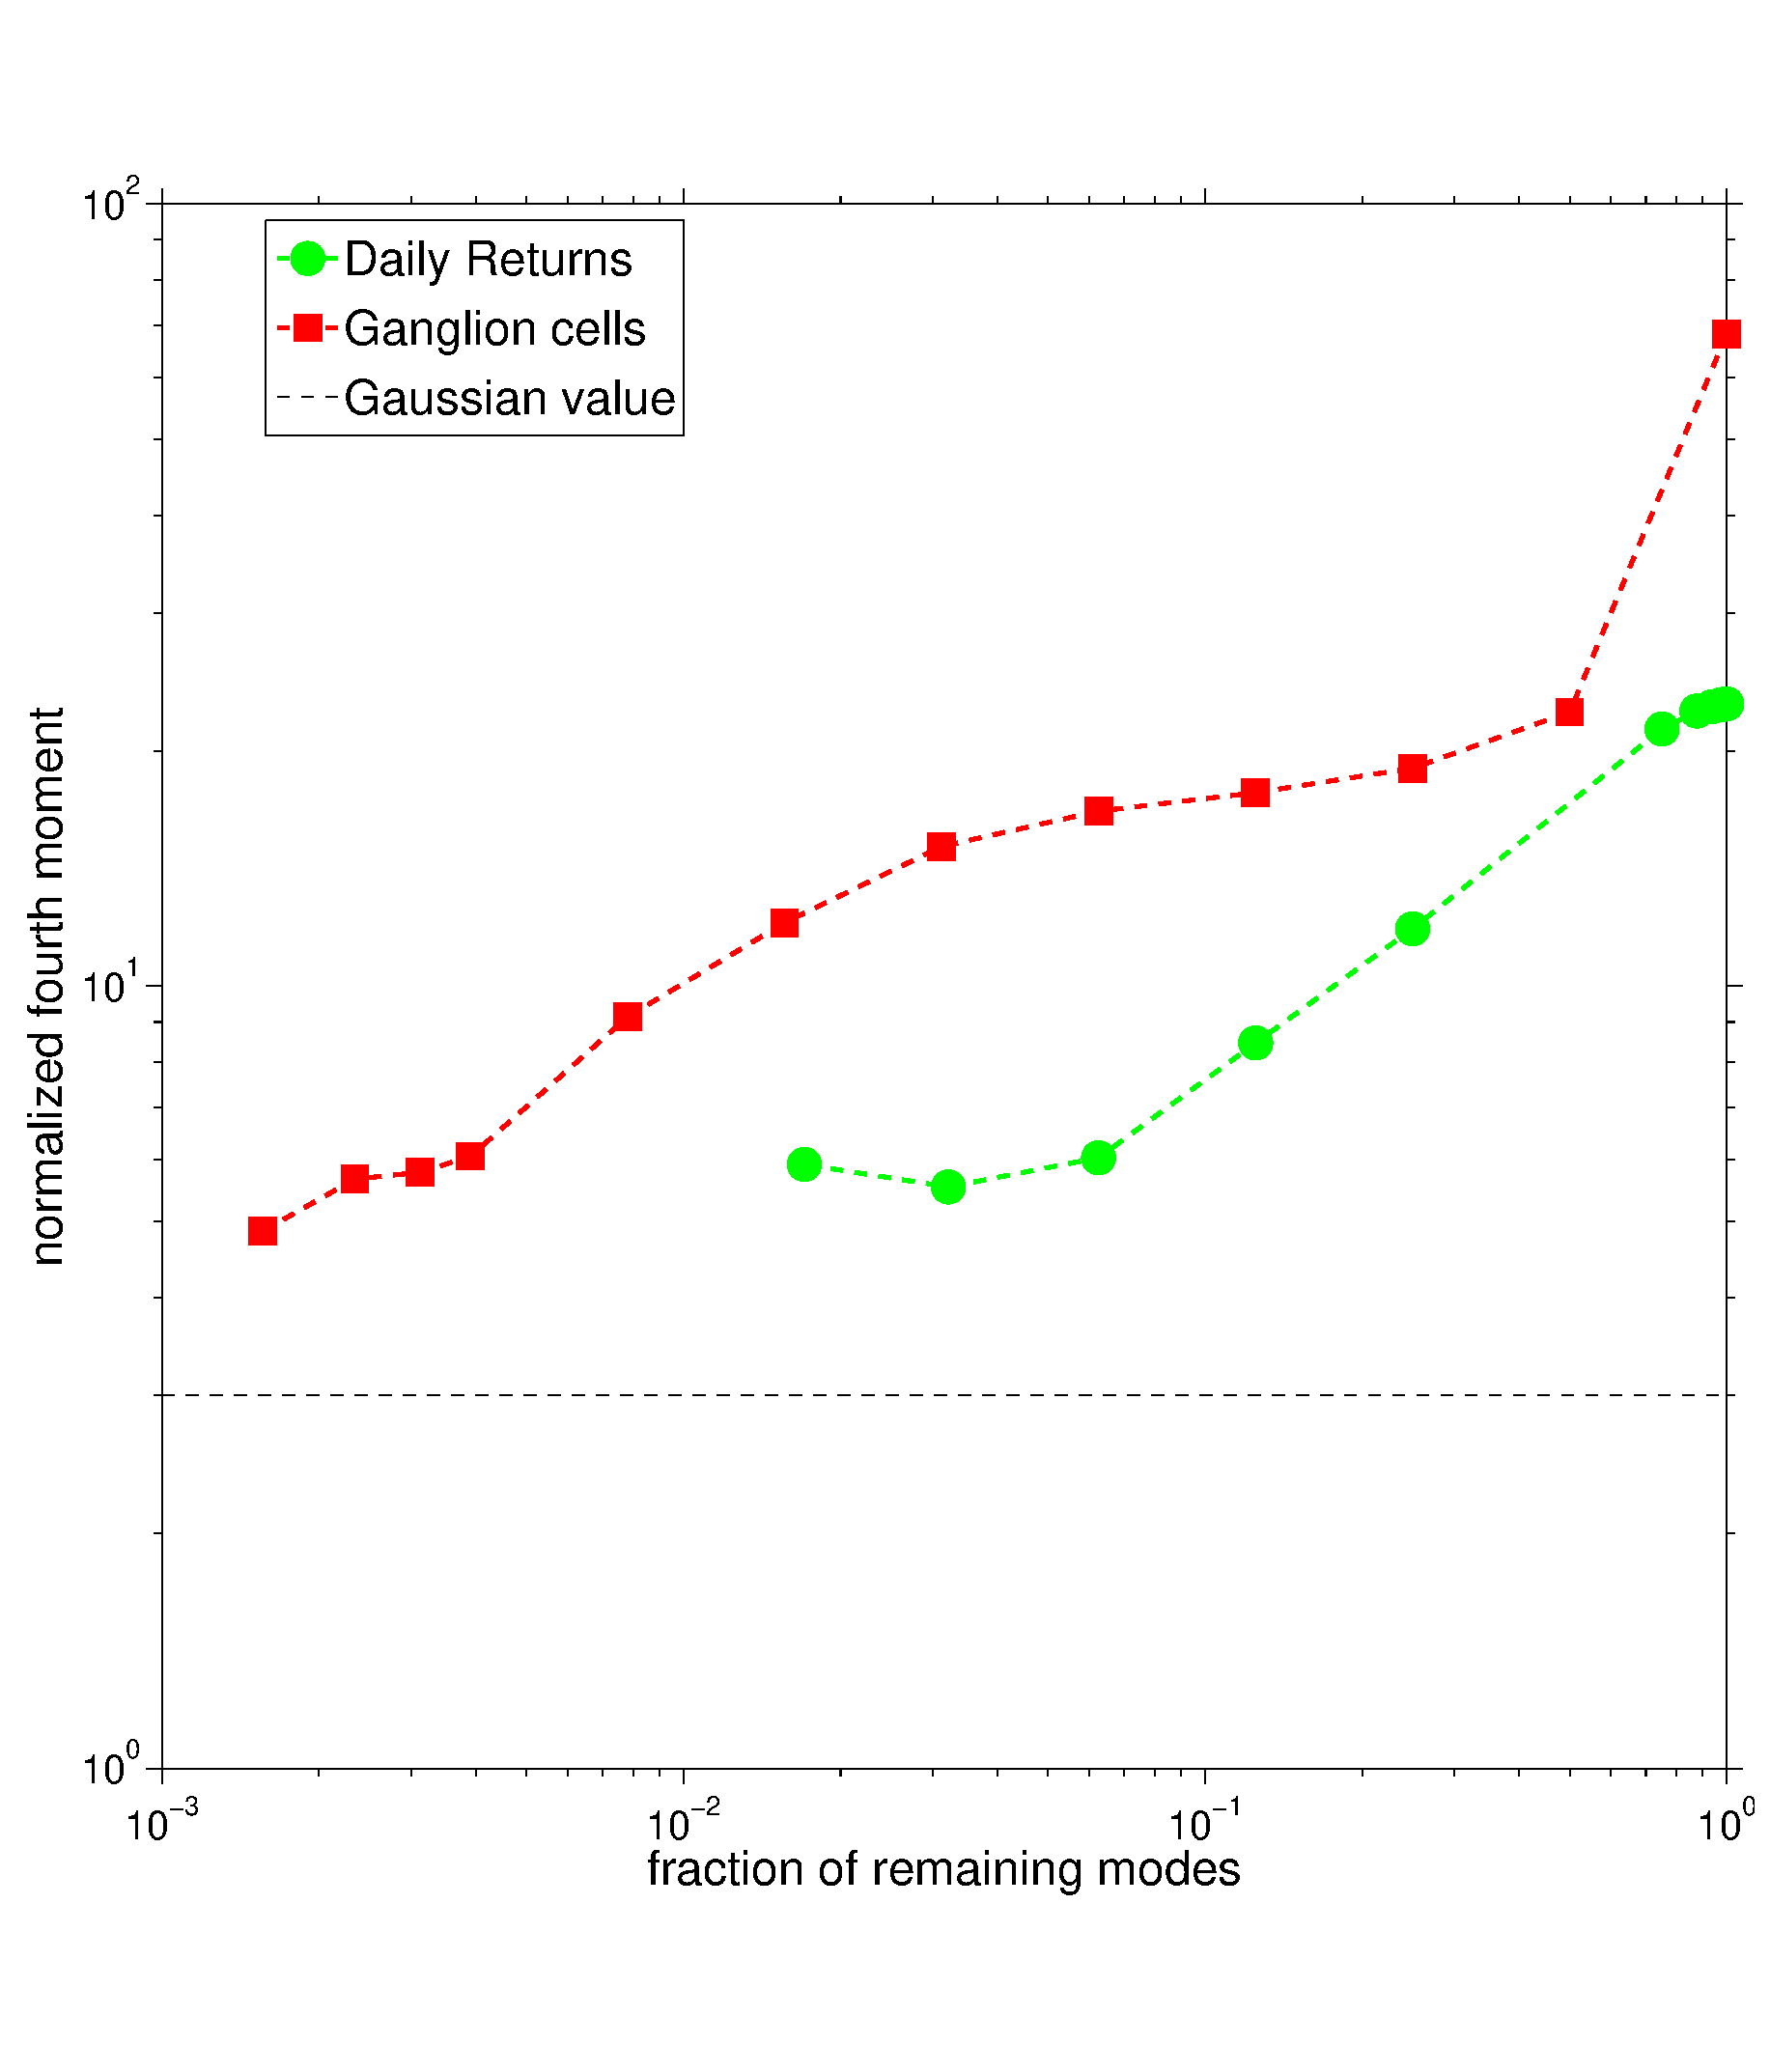
\includegraphics[width=.45\textwidth]{fig2.eps}
\caption{We plot the normalized fourth order correlation, $\sum_i \langle \phi_i^4\rangle/\langle \phi_i^2\rangle^2$, projected on a fraction of eigenmodes, $\lambda<\Lambda$ for two systems: neurons in retina of the salamandra (red) and in daily returns of stocks in the financial market (green). We expect that the fourth order correlation function will reach its gaussian value (dashed black line) if the system is gaussian while if there exist a non-trivial fixed point, the value of fourth order moment deviates from 1/3.}
\label{fig:4th}
\end{figure}

If we remember that the probability distribution $\rho(\lambda )$ is normalized, and choose units where the mean variance of the individual variables is fixed and equal to one, then Eq (\ref{dG4}) simplifies to give ${d\ln \tilde g_{\rm i} }/{d\ln\Lambda} \propto 2-\Lambda$.  As a sanity check, we note that if $\rho(\lambda ) = A  \lambda^{{D/2}-1} $, then to enforce these two normalization conditions we must have $A = D/(2\Lambda^{D/2})$ and $\Lambda = D/(D-2)$, so that $2-\Lambda \propto D-4$. This normalization will be useful in what follows.

%Not sure this is instructive. A correlation matrix has to satisfy several constraints to be a correlation...

%If each individual variable has unit variance, then the matrix $C_{\rm ij}$ is the matrix of correlation coefficients, and  $\Lambda$ is the inverse of the smallest eigenvalue of this matrix.  The mean eigenvalue is one, so large $\Lambda$ corresponds to a wide range of eigenvalues, which are generated by strong correlations.  As an example, if the correlation coefficients are random numbers with standard deviation $\delta C = c/\sqrt{N}$, then for large $N$ random matrix theory tells us that $\Lambda = 1/(1-2c)$.   This suggests that, for weakly correlated systems, with $\delta C < 1/(4\sqrt{N})$, the Gaussian description can be self--consistent, in that small quartic corrections are irrelevant in the RG sense.  On the other hand, for $\delta C > 1/(4\sqrt{N})$ these corrections are relevant, so that non--Gaussianity is always important for systems that reach this level of correlation. 

Thus far our analysis has been confined to ``power counting.''  The next step is to actually integrate out the the low variance degrees of freedom and compute corrections to the coupling constants that are beyond those generated from the spectrum of eigenvalues itself.  Since we can think about discrete modes, we can write $\phi_{\rm i} \rightarrow \phi_{\rm i} + u_{\rm i}(\Lambda)  \psi$, where $\psi$ is the variable describing fluctuations in the ``last mode'' that we have kept in our description, and we want to average over these fluctuations;  in the limit of small $g$,  $\psi$ is Gaussian with $\langle \psi^2\rangle = 1/\Lambda$, and we find
\begin{widetext}
\begin{eqnarray}
\exp\left[ - \frac{1}{4!} N_{\rm eff} \sum_{\rm i} \tilde g_{\rm i}z_\Lambda^4 \phi_{\rm i}^4\right]
&&\rightarrow 
{\bigg\langle}\exp\left[ - \frac{1}{4!} N_{\rm eff} \sum_{\rm i} \tilde g_{\rm i}z_\Lambda^4 (\phi_{\rm i} + u_{\rm i}  \psi)^4\right]{\bigg\rangle}\\
&&\hskip -1in =  \exp\left[ - \frac{1}{2} N_{\rm eff} \sum_{\rm i} \tilde g_{\rm i}z_\Lambda^4 {{u_{\rm i}^2 }\over \Lambda} \phi_{\rm i}^2
 - \frac{1}{4!} N_{\rm eff} \sum_{\rm i} \tilde g_{\rm i}z_\Lambda^4 \phi_{\rm i}^4\
 + \frac{1}{4!} N_{\rm eff}^2 \sum_{{\rm i},{\rm j}} \frac{\tilde g_{\rm i}\tilde g_{\rm j}z_\Lambda^8}{\Lambda^2}  \left[ \frac{3}{2}\phi_{\rm i}^2 \phi_{\rm j}^2 u_{\rm i}^2 u_{\rm j}^2 + \phi_{\rm i}^3 \phi_{\rm j} u_{\rm i} u_{\rm j}^3\right] + \cdots \right] \nonumber\\
 &&
\end{eqnarray}
\end{widetext}

The first term is a correction to the matrix $K$, analogous to a mass renormalization. In the general case all modes get a correction that depends on the local field $\phi_i$. If we assume
that the field is constant and drop the dependence on the index $\rm i$, from the third term, we get that
\begin{equation}
\tilde g \to \tilde g - \frac{3}{2} \tilde g^2 z_\Lambda^4 {{(\sum_i u_{\rm i}^2)^2 }\over {\Lambda^2}} =\tilde g - \frac{3}{2} \tilde g^2 \frac{z_\Lambda^4}{\Lambda^2}
\end{equation}
where we use the condition (\ref{eqn:eigvect}) and normalization condition on the eigenvectors. Notice that we have integrated out exactly one mode, which corresponds to a shift in the cutoff by an amount $d\Lambda$ such that $\rho(\Lambda)d\Lambda =-1$, so we can write
\begin{equation}
d \tilde g=  \frac{3}{2}\rho(\Lambda)  z_\Lambda^4 \tilde g^2 {{d\Lambda} \over {\Lambda^2}} .
\end{equation}
This will reduce to the usual RG calculation if we consider the integration over a shell of momenta and not just the last eigenmode. So we can write
\begin{equation}
d \tilde g =  \frac{3}{2}\rho(\Lambda)  z_\Lambda^4 \tilde g^2    {{d\Lambda} \over {\Lambda^2}} .
\end{equation}
If we combine these perturbative effects with the dimensional effects from Eq (\ref{dG4}),  we have
\begin{equation}
\frac{d\ln \tilde g}{d\ln\Lambda} = \rho(\Lambda) \left[  2   - \Lambda +    \frac{3}{2}  { \tilde g \over \Lambda} \right] \,.
\end{equation}
Since we are  decreasing the cutoff $\Lambda$, this flow generate a stable fixed point at $\tilde g  =0$ for $\Lambda < 2$, or at 
\begin{equation}
\tilde g^* = \frac{2}{3} \Lambda (\Lambda - 2)
\label{fixedpoint}
\end{equation}
for $\Lambda > 2$.
Equation (\ref{fixedpoint}) for the fixed point of the flow may look a bit odd, since it has an explicit dependence on the cutoff, but remember that we have chosen units in which the average variance of the individual degrees of freedom is equal to one, so as we move the cutoff we have to rescale the eigenvalues themselves.  As noted above, in the usual case of local interactions with $-\nabla^2$ in place of the matrix $K_{\rm ij}$, this fixes $\Lambda = D/(D-2)$, and hence $\tilde g^* \propto 4 -D$, as usual. 
We should expect thus that the value $\sum_{\rm i}\langle \phi_{\rm i}^4\rangle /\langle \phi_{\rm i}^2\rangle \to 1/3$ when $\Lambda<2$ and deviates from the gaussian estimate in the opposite regime, $\Lambda>2$. In Fig.\ref{fig:4th} we plot two different examples: the first is the normalized fourth moment of daily return of market stocks and the second is the normalized fourth moment of salamandra retinal ganglion cells recorded at different time. It has been shown that the daily returns of market stocks are well approximated by just few principal components that lies above a given threshold and a noisy bulk below this threshold of variance. If the assumption is correct, we should see that the fourth moment approach its gaussian value as soon as we lower the eigenvalue cutoff below a threshold. In the case of ganglion cells instead, there is no clear evidence that this cutoff exists. This turns into a very different behavior of the fourth moment shown in Fig. \ref{fig:4th}.

In full generality, when the system is not translational invariant, the order parameter depends on the site so we can not drop the index ${\rm i}$. This implies that different interaction terms get different contributions as a correction to $\tilde g_{\rm i}$...

%%%%Serena: SHOULD WE ADD THE CALCULATION commented below??? 

%%CONCLUSION




%THIS ARE THE CALCULATION FOR g_i
%In general, when the system is not translational invariant and the order parameter depends on the site,  we can absorb the ${\rm i} = {\rm j}$ contributions as a correction to $\tilde g_{\rm i}$,
%\begin{equation}
%\tilde g_{\rm i} \rightarrow 
%\tilde g_{\rm i} - \frac{5}{2} N_{\rm eff} \tilde g_{\rm i}^2 z_\Lambda^4 {{u_{\rm i}^4 }\over {\Lambda^2}} \,,
%\end{equation}
%so we can write
%\begin{equation}
%d \tilde g_{\rm i} =  \frac{5}{2}\rho(\Lambda)  z_\Lambda^4 \tilde g_{\rm i}^2 \left(N_{\rm eff} u_{\rm i}^2\right)^2  {{d\Lambda} \over {\Lambda^2}} .
%\end{equation}
%If we combine these perturbative effects with the dimensional effects from Eq (\ref{dG4}),  we have
%\begin{equation}
%\frac{d\ln \tilde g_{\rm i} }{d\ln\Lambda} =   \rho(\Lambda) \left[  2   - \Lambda +    \frac{5}{2} \tilde g_{\rm i} \left(N  u_{\rm i}^2\right)^2  {1\over \Lambda} \right] ,
%\end{equation}
%where we use the normalization conditions above.  We recall from Eq (\ref{normA}) that $\sum_{\rm i}u_{\rm i}^2 = 1$, so that $N  u_{\rm i}^2$ is a number of order unity at large $N$.  Since we are  decreasing the cutoff $\Lambda$, this flow generate a stable fixed point at $\tilde g_{\rm i}  =0$ for $\Lambda < 2$, or at 
%\begin{equation}
%\tilde g_{\rm i}^* = \frac{2}{5}{{\Lambda (\Lambda - 2)}\over{\left(N  u_{\rm i}^2\right)^2 }} 
%\label{fixedpoint}
%\end{equation}
%for $\Lambda > 2$.
%Equation (\ref{fixedpoint}) for the fixed point of the flow may look a bit odd, since it has an explicit dependence on the cutoff, but remember that we have chosen units in which the average variance of the individual degrees of freedom is equal to one, so as we move the cutoff we have to rescale the eigenvalues themselves.  As noted above, in the usual case of local interactions with $-\nabla^2$ in place of the matrix $K_{\rm ij}$, this fixes $\Lambda = D/(D-2)$, and hence $\tilde g_{\rm i}^* \propto 4 -D$, as usual. 






%\cite{fisher+wilson_72}.
%\textcolor{red}{[Can we think about this as the threshold level of correlation needed to evade the central limit theorem?]}
%\textcolor{red}{[Should we do the $c-1/4$ expansion, by analogy with $4-d$?  Do we need examples?  Certainly need to compute the $g^2$ term in the $\beta$ function, so as not to leave the discussion purely at the Gaussian level ... Would be useful to be more explicit about what we are doing now:  integrate out modes with the largest $\lambda$, rescale the variables, rescale the log(probability) to be proportional to $N_{\rm eff}$.]}


\begin{acknowledgments}
We thank \textcolor{red}{[***]}.
Work at CUNY was supported in part by the Swartz Foundation.  Work at Princeton was supported in part by grants from the National Science Foundation (PHY--1305525, PHY--1451171, and CCF--0939370) and the Simons Foundation.
\end{acknowledgments}

%
\begin{thebibliography}{99}
%
%\bibitem{maxent_note}
%It may be useful to note that the probability distribution in Eq (\ref{P1}) is the maximum entropy, and hence least structured,  model consistent with the full covariance matrix and the kurtosis  of each individual variable. 
%%
%\bibitem{fisher+wilson_72}
%KG Wilson and ME Fisher, Critical exponents in 3.99 dimensions. {\em Phys Rev Lett} {\bf 28,} 240--243 (1972).
\end{thebibliography}


\end{document}







